% !TEX encoding = UTF-8 Unicode

\chapter{Tensorflow Implementation}
\label{chap:implementation}

%%%%%%%%%%%%%%%%%%%%%%%%%%

\section{System overview}
\label{sec:implementation:overview}

The style transfer system is implemented mainly with Python Tensorflow,
with auxiliary packages including NumPy, SciPy, and Pillows.
A flowchart of the system overview is provided in Fig.\,~\ref{fig:overview}.

    \begin{figure}[!hbt]
    \center
    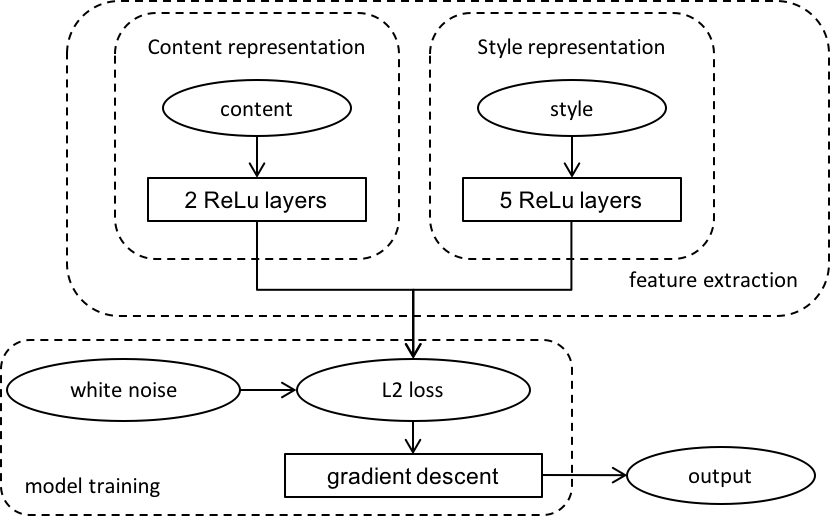
\includegraphics[width=0.8\textwidth]{overview.png}
    \caption{Tensorflow implementation system overview}
    \label{fig:overview}
    \end{figure}

In feature extraction part, the pre-trained VGG network is used for both
content representation and style representation.
One ReLu layers (relu4\_2) is for content feature extraction
and five ReLu layers (relu1\_1, relu2\_1, relu3\_1, relu4\_1, relu5\_1) are for 
stye representation, which are different from the original work \cite{Gatys:2016gj}.

In model training part, the final output is initialized with a white noise picture,
and a gradient-based optimization methodology known as Adam is used.
As is described in \cite{kingma2014adam}, Adam optimizer is based on first-order gradient.
Other optimizers including traditional gradient descent method can also be implemented.

%%%%%%%%%%%%%%%%%%%%%%%%%%

\section{Pre-defined parameters}

Some tuning parameters are hard-wired in the system.
Most of the choices follow the original work \cite{Gatys:2016gj},
or the reference \cite{athalye2015neuralstyle} and some are modified.

There is plenty of room with cross-validatio optimization for performace improvement
(see Sec\,~\ref{sec:discussion:parameter} for more details).
For simplicity, they are fixed in this system for now and the user can easily modify part of them
in \texttt{constants.py} following instruction in \ref{app:readme}.

Some pre-defined parameters are listed below in Table \ref{table:parameters}.
The ratio of content loss and style loss is arbitrarily set while \cite{Gatys:2016gj}
explores different loss ratios and corresponding output results.
Parameters can always be modified and optimized with techniques like cross-validation.

	\begin{table}[!htb]
	\center
	\begin{tabular}{c|c}
	\hline
	parameter type & parameter value \\ \hline
	content weight & 5 \\
	style weight & 500 \\
	total variation weight & 100 \\
	Adam learning rate & 10 \\
	Adam $\beta_1$ & 0.9 \\
	Adam $\beta_2$ & 0.999 \\
	Adam $\epsilon$ & $10^{-8}$ \\
	maximum iteration & 1000 \\
	pooling layer method & max \\
	\hline
	\end{tabular}
	\caption{Pre-defined model parameters}
	\label{table:parameters}
	\end{table}

Apart from model parameters, neural network choice in this work is also different.
	
	\begin{table}[!htb]
	\center
	\begin{tabular}{c|c|l}
	\hline
	& & \multicolumn{1}{c}{layers used} \\ \hline
	\multirow{3}{*}{content representation}
		& this work & relu4\_2 \\
		& original work & conv1\_1, conv4\_2 \\
		& Anish work & relu4\_2, relu5\_2 (weight adjustable) \\ \hline
	\multirow{3}{*}{style representation}
		& this work & relu1\_1, relu2\_1, relu3\_1, relu4\_1, relu5\_1 \\
		& original work & conv1\_1, conv2\_1, conv3\_1, conv4\_1, conv5\_1 \\
		& Anish work & relu1\_1, relu2\_1, relu3\_1, relu4\_1, relu5\_1 \\
	\hline
	\end{tabular}
	\caption{Pre-defined feature extraction layers}
	\label{table:layers}
	\end{table}

Specifically, all layers in style representation are equally weighted.
The random initialization, i.e.\ process to generate the white noise graph
is arbitrary as well but has little impact on the output results,
and thus is omitted here.
